%\documentclass[tikz,border=3mm]{standalone}
%\begin{document}

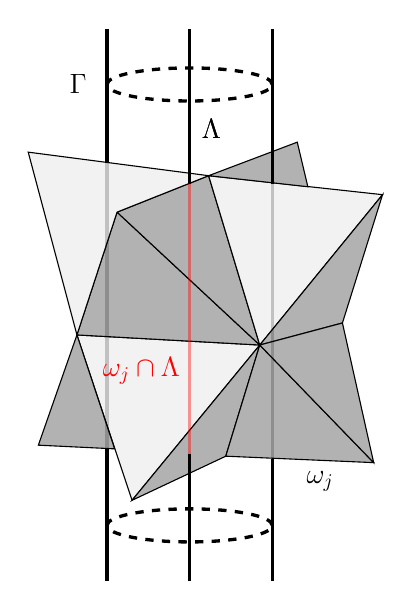
\begin{tikzpicture}[scale=0.7, every node/.style={scale=0.7}]
\pgfmathsetmacro{\factor}{1/sqrt(2)};
\coordinate  (A) at (2,0,-1*\factor);
\coordinate  (B) at (2.2,-1.2,2*\factor);
\coordinate  (C) at (-0.5,1,2*\factor);
\coordinate  (D) at (0.5,-2,2*\factor);
\coordinate  (E) at (0.5,3.5,3*\factor);
\coordinate  (F) at (0.8,2.8,-2*\factor);
\coordinate  (G) at (-1.2,-1,2*\factor);
\coordinate  (H) at (5.7,-0.5,5*\factor);
\coordinate  (I) at (1,-0.25,5*\factor);
\coordinate  (L) at (-2.5,3.2,-2.1*\factor);
\coordinate  (M) at (4.5,3,0*\factor);
\coordinate  (N) at (3.5,0.4,-1*\factor);
\coordinate  (O) at (2,3,-3.5*\factor);
\coordinate  (P) at (2.6,2.6,-2*\factor);
%\draw[->] (0,0) -- (3,0,0) node[right] {$x$};
%\draw[->] (0,0) -- (0,3,0) node[above] {$y$};
%\draw[->] (0,0) -- (0,0,3) node[below left] {$z$};
%\foreach \i in {A,B,C,D}
%\draw[dashed] (0,0)--(\i);
\draw[black, fill=white!90!gray] (A)--(D)--(C)--cycle;
\draw[black,  fill=gray!60!] (A) --(B)--(D)--cycle;
\draw[black, fill=gray!60!] (E) --(C)--(A)--cycle;
\draw[black,   fill=gray!60!] (E) --(F)--(A)--cycle;
\draw[black,    fill=gray!60!] (B) --(A)--(H)--cycle;
\draw[black,    fill=gray!60!] (C) --(G)--(I)--cycle;
\draw[black, fill=white!90!gray] (C) -- (E) -- (F)--(L)--cycle;
\draw[black,  fill=white!90!gray] (A) --(F)--(M)--cycle;
\draw[black,   fill=gray!60!] (A) --(N)--(M)--cycle;
\draw[black,    fill=gray!60!] (A) --(N)--(H)--cycle;
\draw[black,    fill=gray!60!] (F) --(O)--(P)--cycle;
%\draw[-, fill=gray!30!blue, opacity=.2] (E) --(G)--(H)--cycle;
\node [font=\Large, right] at (3, -2.2) {$\omega_j$};


%cylinder Gamma
\draw[dashed, very thick] (1, 5) ellipse (1.5 and 0.3);
\draw[dashed, very thick] (1, -3) ellipse (1.5 and 0.3);
\draw[black, very  thick] (-0.5, 3.6) -- (-0.5, 6);
\draw[black, very thick, opacity=.2] (-0.5, 3.6) -- (-0.5, -1.6);
\draw[black, very  thick] (-0.5, -1.6) -- (-0.5, -4); 
\draw[ very thick] (2.5, 6) -- (2.5, 3.2);
\draw[ very thick, opacity =0.2] (2.5, 3.2) -- (2.5, -1.8);
\draw[very thick] (2.5, -1.8) -- (2.5, -4);
\node [font=\Large, right] at (-1.3, 5) {$\Gamma$};

%centerline \Lambda
\draw[very thick] (1, 6) -- (1, 3.2);
\draw[red, very thick, opacity=.4] (1, 3.2) -- (1, -1.8);
\draw[very thick, ]  (1, -1.7) -- (1, -4);
\node [font=\Large, right] at (1.1, 4.2) {$\Lambda$};
\node [font=\Large, right] at (1.1, 4.2) {$\Lambda$};
\node [font=\Large, right, red] at (-0.7, -0.2) {$\omega _j \cap \Lambda$};
\end{tikzpicture}



%\end{document}